\chapter[Longest Palindromic Substring]
{Longest Palindromic Substring
  \label{chLngstPlndrmcSbstrng}}
\chaptermark{Longest Palindromic Substring}


\begin{itemize}%[noitemsep,topsep=0pt]
\item My own attempt.
\item Longest Palindromic Substring | Set 1:
  \url{https://www.geeksforgeeks.org/longest-palindrome-substring-set-1}
\item Longest Palindromic Substring | Set 2:
  \url{https://www.geeksforgeeks.org/longest-palindromic-substring-set-2}
\item Manacher's Algorithm -- Linear Time Longest Palindromic Substring --
  Part 1:
  \url{https://www.geeksforgeeks.org/manachers-algorithm-linear-time-longest-palindromic-substring-part-1}
\item Manacher's Algorithm -- Linear Time Longest Palindromic Substring --
  Part 2:
  \url{https://www.geeksforgeeks.org/manachers-algorithm-linear-time-longest-palindromic-substring-part-2}
\end{itemize}


% for Longest Palindromic SubSEQUENCE, we will use
% secLPSSeq
\section{My Attempt\label{secLPSStrMyAttempt}}

\url{https://leetcode.com/problems/longest-palindromic-substring/description}

Given a string $s$, find the longest palindromic substring in $s$. You may
assume that the maximum length of $s$ is 1000.

\noindent{}\textbf{Example:}
\begin{lstlisting}[style=raygeneric]
Input: "babad"
Output: "bab"
Note: "aba" is also a valid answer.
\end{lstlisting}
\noindent{}\textbf{Example:}
\begin{lstlisting}[style=raygeneric]
Input: "cbbd"
Output: "bb"
\end{lstlisting}

\qasepline{}

Note that this asking for a substring, not a subsequence.
For a subsequence, we'll have to use a DP approach from both ends, so that
\begin{lstlisting}[style=raygeneric]
LPS(s[1..n]) = if s[1]==s[n]
                 LPS(2..n-1)+2
               else
                 max(LPS(i+1..j), LPS(i..j-1))
\end{lstlisting}
See http://www.geeksforgeeks.org/dynamic-programming-set-12-longest-palindromic-subsequence
Okay, we'll continue with the solution.

\qasepline{}

We take advantage of the fact that we're dealing with substrings. This means
that the characters need to be consecutive (unlike in a subsequence).  Since
characters in a substring are consecutive. Say is we have string
$s=[0..i..j..n]$, then the LPS ending at $j$ is either
\begin{itemize}%[noitemsep,topsep=0pt]
\item 1 (the character itself)
\item or it includes the character before it.
\end{itemize}
If it includes the character before it, then it must include the max length
palindrome ending at $j-1$. I.e.
\begin{lstlisting}[style=raygeneric]
[0..i,(i+1)..(j-1),j..n]
\end{lstlisting}
then $s=[(i+1)..(j-1)]$ must also be a palindrome, which we have calculated
previously. What's the base case? At $s[0]$, we have a palindrome of
$LPS[0]=1$. At
\ctt{s[j]}, it's \ctt{LPS[j]} is max of $1$ or if \ctt{s[j]==s[ j-LPS[j-1]-1
  ]}, then equals to \ctt{LPS[j-1]+2}. However, if $j-LPS[j-1]-1<0$, then
it's $1$.
\begin{lstlisting}[style=raygeneric]
s[0 1 2 3   4 5   6 7 8]
L[    i i+1   j-1 j    ]
              3   ?
\end{lstlisting}
Also, we need to keep track of the index of max LPS, so we can extract the
string from s.

Actually, this won't work for the simple case of "\ctt{s=[aaaaaaa]}", since
at any $s[j]$, the length of the LPS before it, $LPS[j-1]$ goes all the way
to the beginning. Thus, it will try to compare $s[j]$ to one before the
beginning of $s$, which is impossible, so it'll say the LPS of $j$ is $1$,
but it's not.

\qasepline{}

Okay, that approach won't work, and I can't think of a way to make it work.
However, I have noticed another way. The substring $s[i..j]$ is a palindrome
is and only if $s[i]==s[j]$ AND $s[i+1..j-1]$ is a palindrome. So what we
can do is have a table $dp[N-1][N-1]$, where $N=s.size()$, and let
$dp[i][j]$ be the length of the palindrome $s[i..j]$ or $0$ is it isn't a
palindrome. If $dp[i][j]$ is a palindrome, then it must be that
$dp[i+1][j-1]$ is a palindrome. So:
\begin{lstlisting}[style=raygeneric]
dp[i][j] = if(s[i]==s[j] && dp[i+1][j-1]>0)
             dp[i+1][j-1]+2
           else 0
\end{lstlisting}
The \textbf{base case}, every character is a palindrome of length $1$, so
$dp[i][i]=1$ for $i=0..N$. How do we iterate through the $dp$ table? We see
from the recurrent relation that $(i,j)$ depends on $(i+1,j-1)$, and $j>i$.
Let's see how the recursion works for $(i=1,j=2)$, this depends on $(2,1)$,
which is impossible. This is because we need $j>i$, and at each step, we
increase $i$ and decrease $j$, which means that we need to explicitly fill
in substrings of length = 2.
\begin{lstlisting}[style=raygeneric]
  0 1 2 3 4
  ----------
0|1 X Y Z ?
1|  1 X Y Z
2|    1 X Y
3|      1 X
4|        1
\end{lstlisting}
Okay so, let's work with the lengths, going from $l=0..N-1$. If $l=1$, then
$dp[i][j]=1$. If $l=2$, then $dp[i][j]=2$ if ($s[i]==s[j]$). For $l>=3$, we
have the relationship:
\begin{equation*}
l=j-i+1
\end{equation*}
I.e.
\begin{lstlisting}[style=raygeneric]
0 1 2 3 4 5 6
a b c d e f g
    i     j
\end{lstlisting}
length of $(i=2,j=5)=5-2+1=4$. For each $l$, we need to work out $i$ and
$j$. Looking at the dp table above, we see:
\begin{lstlisting}[style=raygeneric]
N=5
l=1, i=0..N-1=4
l=2, i=0..N-2=3
l=3, i=0..N-3=2
\end{lstlisting}
so $i=0..N-l$, and from the equation, $j=l+i-1$.  This is how we'll fill in
our table. Now, we also need to keep track of the max length palindrome
index so I can extract it later. Let's code this up. Code is here:
\path{Algorithms/5LngstPlndrmcSbstrng/rrrMain.cpp}
\begin{lstlisting}[style=raycppnewsnippet]
template<typename T>
using Grid2d = vector<vector<int>>;

void solveLPSDP(const string& str)
{
  auto N = static_cast<int>(str.size());
  Grid2d<int> grid(N,vector<int>(N,0));

  // base case when one char
  for(int i = 0; i < N; ++i)
    grid[i][i]=1;

  int maxLPSLen=1;
  int maxi=0;
  int maxj=0; // This is important as well, start with maxi=maxj=0 for l=1.
  // Start at length l = 2
  // This is the LENGTH, which INCLUDES N
  for(int l=2; l <= N; ++l)
  {
    // Loop through rows, i=0..N-l
    for(int i = 0; i < (N-l+1); ++i) // +1 was another bug I forgot to add..
    {
      // calculate j
      int j = l+i-1;

      // if l=2, check if palindrome
      if(l==2 && str[i]==str[j])
      {
        grid[i][j]=2;
      }
      else
      {
        if(str[i]==str[j] && grid[i+1][j-1] > 0)
        {
          grid[i][j]= 2+grid[i+1][j-1];
        }
      }

      // Update if LPS.
      if(grid[i][j]>maxLPSLen)
      {
        maxLPSLen=grid[i][j];
        maxi = i; maxj = j;
      }
    }
  }
  // C++ algos works with on past the end, also, substr's second param is
  // the count of the letters. We need to +1 cos this is an inclusive range
  // i.e. [i..j] should include all the chars from i to j, so we need to +1
  // to get the total number of chars. If this was [i..j), then j-i would
  // give the total number of chars
  cout << str.substr(maxi, (maxj-maxi+1)) << '\n';
}
\end{lstlisting}
Okay, this works, let's see what Leetcode has to say:

\subsection{Longest Palindromic Substring LC Solution}

This article is for intermediate readers. It introduces the following ideas:
Palindrome, Dynamic Programming and String Manipulation. Make sure you
understand what a palindrome means. A palindrome is a string which reads the
same in both directions. For example, \ctt{``aba''} is a palindrome,
\ctt{``abc''} is not.

\rrheader{Approach \#1 (Longest Common Substring) [Accepted]}

\noindent{}\textbf{Common mistake}
Some people will be tempted to come up with a quick solution, which is
unfortunately flawed (however can be corrected easily):
\begin{mdframed}[style=mdfNOTE]
Reverse $S$ and become $S'$. Find the longest common substring between $S$
and $S'$, which must also be the longest palindromic substring.
\end{mdframed}
This seemed to work, let's see some examples below.
\begin{itemize}%[noitemsep,topsep=0pt]
\item For example, $S=[caba]$, $S'=[abac]$. The longest common substring
  between $S$ and $S'$ is $aba$, which is the answer.
\item Let's try another example: $S=[abacdfgdcaba]$, $S'=[abacdgfdcaba]$.

The longest common substring between $S$ and $S'$ is \ctt{abacd}. Clearly,
this is not a valid palindrome.
\end{itemize}

\noindent{}\textbf{Algorithm}

We could see that the longest common substring method fails when there
exists a reversed copy of a non-palindromic substring in some other part of
S. 
\begin{lstlisting}[style=raygeneric]
 S=[@@abacd@@fg@@dcaba@@]
S'=[@@abacd@@gf@@dcaba@@]
\end{lstlisting}
To rectify this, each time we find a longest common substring candidate, we
check if the substring's indices are the same as the reversed substring's
original indices. If it is, then we attempt to update the longest palindrome
found so far; if not, we skip this and find the next candidate.

This gives us an $\comBigOh{n^2}$ Dynamic Programming solution which uses
$\comBigOh{n^2}$ space (could be improved to use $\comBigOh{n}$ space).
Please read more about Longest Common Substring
here\footnote{\url{https://en.wikipedia.org/wiki/Longest\_common\_substring\_problem}}.


\rrheader{Approach \#2 (Brute Force) [Time Limit Exceeded]}

The obvious brute force solution is to pick all possible \textbf{starting}
and \textbf{ending} positions for a substring, and verify if it is a
palindrome.

\noindent{}\textbf{Complexity Analysis}
\begin{itemize}%[noitemsep,topsep=0pt]
\item Time complexity: $\comBigOh{n^3}$. Assume that $n$ is the length of
  the input string, there are a total of $\binom{n}{2}=\frac{n(n-1)}{2}$
  such substrings (excluding the trivial solution where a character itself
  is a palindrome). Since verifying each substring takes $\comBigOh{n}$
  time, the run time complexity is $\comBigOh{n^3}$.
\item Space complexity: $\comBigOh{1}$.
\end{itemize}

\rrheader{Approach \#3 (Dynamic Programming) [Accepted]}

\rrblue{(This is the one I came up with)}

To improve over the brute force solution, we first observe how we can avoid
unnecessary re-computation while validating palindromes. Consider the case
\ctt{ababa}. If we already knew that \ctt{bab} is a palindrome, it is
obvious that \ctt{ababa} must be a palindrome since the two left and right
end letters are the same.

We define $P(i,j)$ as following:
\begin{equation*}
P(i,j)=
\begin{cases}
\text{true} &\text{ if the substring $S_i\ldots S_j$ is a palindrome,}\\
\text{false}&\text{ otherwise.}
\end{cases}
\end{equation*}
Therefore
\begin{equation*}
P(i,j)=(P(i+1,j-1) \text{and} S_i==S_j)
\end{equation*}
The base cases are:
\begin{align*}
P(i,j) &= \text{true}\\
P(i,i+1)&= (S_i == S_{i+1})
\end{align*}
This yields a straight forward DP solution, which we first initialize the
one and two letters palindromes, and work our way up finding all three
letters palindromes, and so on...

\noindent{}\textbf{Complexity Analysis}
\begin{itemize}[noitemsep,topsep=0pt]
\item Time complexity: $\comBigOh{n^2}$. This gives us a runtime complexity
  of $\comBigOh{n^2}$.
\item Space complexity: $\comBigOh{n^2}$. It uses $\comBigOh{n^2}$ space to
  store the table.
\end{itemize}

\noindent{}\textbf{Additional Exercise}

Could you improve the above space complexity further and how?

\rrheader{Approach \#4 (Expand Around Center) [Accepted]}

In fact, we could solve it in $\comBigOh{n^2}$ time using only constant
space.

We observe that a palindrome mirrors around its center. Therefore, a
palindrome can be expanded from its center, and there are only $2n-1$ such
centers.

You might be asking why there are $2n-1$ but not $n$ centers \rrblue{(since
  there are $n$ characters)}? The reason
is the center of a palindrome can be in between two letters. Such
palindromes have even number of letters (such as \ctt{abba})
and its center are between the two \ctt{b}s.
\begin{lstlisting}[style=raygeneric]
 1 2 3 4
#a#b#c#f#
123456789
\end{lstlisting}

\rrblue{(I just did this, see the rrrMain.cpp file.)}


\rrheader{Approach \#5 (Manacher's Algorithm) [Accepted]}

There is even an $\comBigOh{n}$ algorithm called Manacher's algorithm,
explained here in
detail\footnote{\url{https://articles.leetcode.com/longest-palindromic-substring-part-ii}}.
However, it is a non-trivial algorithm, and no one expects you to come up
with this algorithm in a 45 minutes coding session. But, please go ahead and
understand it, I promise it will be a lot of fun.


\subsection{Manacher's algorithm}

\noindent{}\textbf{Note:}\\
This is Part II of the article: Longest Palindromic Substring. Here, we
describe an algorithm (Manacher's algorithm) which finds the longest
palindromic substring in linear time. Please read Part I for more background
information.

In my previous post we discussed a total of four different methods, among
them there's a pretty simple algorithm with $\comBigOh{N^2}$ run time and
constant space complexity. Here, we discuss an algorithm that runs in
$\comBigOh{N}$ time and $\comBigOh{N}$ space, also known as Manacher's
algorithm.

\noindent{}\textbf{Hint:}\\
Think how you would improve over the simpler $\comBigOh{N^2}$ approach.
Consider the worst case scenarios. The worst case scenarios are the inputs
with multiple palindromes overlapping each other. For example, the inputs:
``\ctt{aaaaaaaaa}'' and ``\ctt{cabcbabcbabcba}''. In fact, we could take
advantage of the palindrome's symmetric property and avoid some of the
unnecessary computations.

\rrheader{An $\comBigOh{N}$ Solution (Manacher's Algorithm):}

First, we transform the input string, $S$, to another string $T$ by
inserting a special character ``\ctt{\#}'' in between letters. The reason
for doing so will be immediately clear to you soon.

For example: \ctt{S=[abaaba]}, \ctt{T=[\#a\#b\#a\#a\#b\#a\#]}.

To find the longest palindromic substring, we need to expand around each
$T_i$ such that $T_{i-d}\ldots T_{i+d}$ forms a palindrome. You should
immediately see that $d$ is the length of the palindrome itself centered at
$T_i$ \rrblue{(since we have added extra \ctt{\#}s' in)}.

We store intermediate result in an array $P$, where $P[i]$ equals to the
length of the palindrome centers at $T_i$. The longest palindromic substring
would then be the maximum element in $P$.

Using the above example, we populate $P$ as below (from left to right):
\begin{lstlisting}[style=raygeneric]
T = # a # b # a # a # b # a #
P = 0 1 0 3 0 1 6 1 0 3 0 1 0
\end{lstlisting}
Looking at $P$, we immediately see that the longest palindrome is
``\ctt{abaaba}'', as indicated by $P_6=6$.

Did you notice by inserting special characters (\ctt{\#}) in between
letters, both palindromes of odd and even lengths are handled graciously?
(Please note: This is to demonstrate the idea more easily and is not
necessarily needed to code the algorithm.)

Now, imagine that you draw an imaginary vertical line at the center of the
palindrome ``\ctt{abaaba}''. Did you notice the numbers in $P$ are symmetric
around this center? That's not only it, try another palindrome
``\ctt{aba}'', the numbers also reflect similar symmetric property. Is this
a coincidence? The answer is yes and no. This is only true subjected to a
condition, but anyway, we have great progress, since we can eliminate
recomputing part of \ctt{P[i]}'s.

Let us move on to a slightly more sophisticated example with more some
overlapping palindromes, where \ctt{S=[babcbabcbaccba]}.

\begin{figure}
\centering
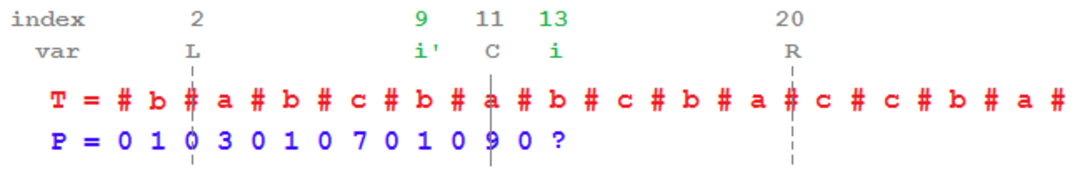
\includegraphics[width=0.95\textwidth]{Images/figLCLngstPlndrmcSubstring1}
\caption{Above image shows \ctt{T} transformed from
  \ctt{S=[babcbabcbaccba]}.  Assumed that you reached a state where table
  \ctt{P} is partially completed. The solid vertical line indicates the
  center (\ctt{C}) of the palindrome \ctt{abcbabcba}. The two dotted
  vertical line indicate its left (\ctt{L}) and right (\ctt{R}) edges
  respectively. You are at index $i$ and its mirrored index around \ctt{C}
  is \ctt{i'}. How would you calculate \ctt{P[i]} efficiently?}
%\label{figCXNX}
\end{figure}

Assume that we have arrived at index $i=13$, and we need to calculate
\ctt{P[13]} (indicated by the question mark \ctt{?}). We first look at its
mirrored index \ctt{i'} around the palindrome's center \ctt{C}, which is
index \ctt{i'=9}.

\begin{figure}
\centering
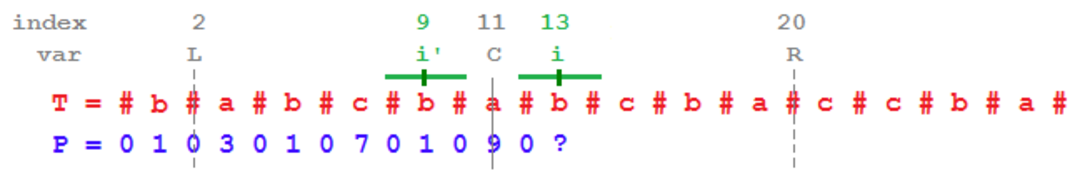
\includegraphics[width=0.95\textwidth]{Images/figLCLngstPlndrmcSubstring2}
\caption{The two green solid lines above indicate the covered region by the
  two palindromes centered at \ctt{i} and \ctt{i'}. We look at the mirrored
  index of \ctt{i} around \ctt{C}, which is index \ctt{i'}.
  \ctt{P[i']=P[9]=1}. It is clear that \ctt{P[i]} must also be \ctt{1}, due
  to the symmetric property of a palindrome around its center.}
%\label{figCXNX}
\end{figure}

As you can see above, it is very obvious that P[ i ] = P[ i' ] = 1, which
must be true due to the symmetric property around a palindrome's center. In
fact, all three elements after C follow the symmetric property (that is, P[
12 ] = P[ 10 ] = 0, P[ 13 ] = P[ 9 ] = 1, P[ 14 ] = P[ 8 ] = 0).

\begin{figure}
\centering
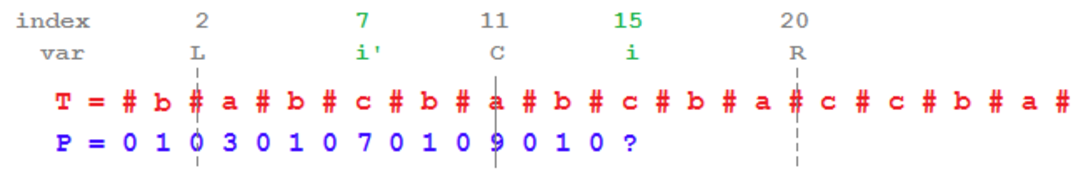
\includegraphics[width=0.95\textwidth]{Images/figLCLngstPlndrmcSubstring3}
\caption{Now we are at index i = 15, and its mirrored index around C is i' = 7. Is P[ 15 ] = P[ 7 ] = 7?}
%\label{figCXNX}
\end{figure}

Now we are at index i = 15. What's the value of P[ i ]? If we follow the
symmetric property, the value of P[ i ] should be the same as P[ i' ] = 7.
But this is wrong. If we expand around the center at T15, it forms the
palindrome “a\#b\#c\#b\#a”, which is actually shorter than what is indicated by
its symmetric counterpart. Why?


\begin{figure}
\centering
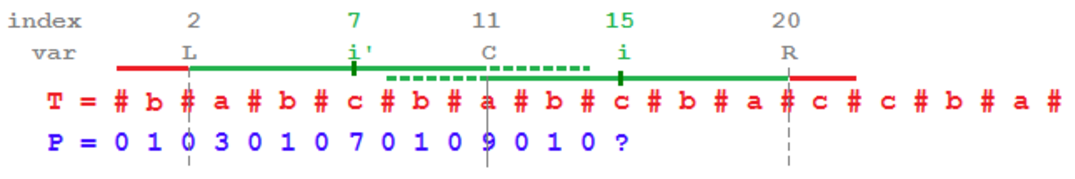
\includegraphics[width=0.95\textwidth]{Images/figLCLngstPlndrmcSubstring4}
Colored lines are overlaid around the center at index i and i'. Solid green lines show the region that must match for both sides due to symmetric property around C. Solid red lines show the region that might not match for both sides. Dotted green lines show the region that crosses over the center.
\caption{}
%\label{figCXNX}
\end{figure}

It is clear that the two substrings in the region indicated by the two solid
green lines must match exactly. Areas across the center (indicated by dotted
green lines) must also be symmetric. Notice carefully that P[ i ' ] is 7 and
it expands all the way across the left edge (L) of the palindrome (indicated
by the solid red lines), which does not fall under the symmetric property of
the palindrome anymore. All we know is P[ i ] geq 5, and to find the real
value of P[ i ] we have to do character matching by expanding past the right
edge (R). In this case, since P[ 21 ] neq P[ 1 ], we conclude that P[ i ] = 5.

Let's summarize the key part of this algorithm as below:

if P[ i' ] leq R - i,
then P[ i ] := P[ i' ]
else P[ i ] geq P[ i' ]. (Which we have to expand past the right edge (R) to find P[ i ].

See how elegant it is? If you are able to grasp the above summary fully, you
already obtained the essence of this algorithm, which is also the hardest
part.

The final part is to determine when should we move the position of C
together with R to the right, which is easy:

If the palindrome centered at i does expand past R, we update C to i, (the
center of this new palindrome), and extend R to the new palindrome's right
edge.

In each step, there are two possibilities. If P[ i ] leq R - i, we set P[ i ]
to P[ i' ] which takes exactly one step. Otherwise we attempt to change the
palindrome's center to i by expanding it starting at the right edge, R.
Extending R (the inner while loop) takes at most a total of N steps, and
positioning and testing each centers take a total of N steps too. Therefore,
this algorithm guarantees to finish in at most 2*N steps, giving a linear
time solution.



%%%%%%%%%%%%%%%%%%%%%%%%%%%%%%%%%%%%%%%%%%%%%%%%%%%%%%%%%%%%%%%%%%%%%%%%%%%%
%%%%%%%%%%%%%%%%%%%%%%%%%%%%%%%%%%%%%%%%%%%%%%%%%%%%%%%%%%%%%%%%%%%%%%%%%%%%
%%%%%%%%%%%%%%%%%%%%%%%%%%%%%%%%%%%%%%%%%%%%%%%%%%%%%%%%%%%%%%%%%%%%%%%%%%%%

\section{Longest Palindromic Substring | Set 1
  \label{secLPSStrGFGLngstPlndrmcSbstrngSet1}}

\url{https://www.geeksforgeeks.org/longest-palindrome-substring-set-1}

\textbf{Difficulty: 3.5}

\textbf{\rrgreen{Recommended: Please try your approach first, before moving
    on to the solution.}}

\RayNotesBegin

I understand already, moving onto Manacher's algorithm

\RayNotesEnd

\textbf{\rrgreen{Back to geeksforgeeks solution.}}





%%%%%%%%%%%%%%%%%%%%%%%%%%%%%%%%%%%%%%%%%%%%%%%%%%%%%%%%%%%%%%%%%%%%%%%%%%%%
%%%%%%%%%%%%%%%%%%%%%%%%%%%%%%%%%%%%%%%%%%%%%%%%%%%%%%%%%%%%%%%%%%%%%%%%%%%%
%%%%%%%%%%%%%%%%%%%%%%%%%%%%%%%%%%%%%%%%%%%%%%%%%%%%%%%%%%%%%%%%%%%%%%%%%%%%

\section{Longest Palindromic Substring | Set 2
  \label{secLPSStrGFGLngstPlndrmcSbstrngSet2}}

\url{https://www.geeksforgeeks.org/longest-palindromic-substring-set-2}

\textbf{Difficulty: 3.2}

\textbf{\rrgreen{Recommended: Please try your approach first, before moving
    on to the solution.}}

\RayNotesBegin

I understand already, moving onto Manacher's algorithm

\RayNotesEnd

\textbf{\rrgreen{Back to geeksforgeeks solution.}}




%%%%%%%%%%%%%%%%%%%%%%%%%%%%%%%%%%%%%%%%%%%%%%%%%%%%%%%%%%%%%%%%%%%%%%%%%%%%
%%%%%%%%%%%%%%%%%%%%%%%%%%%%%%%%%%%%%%%%%%%%%%%%%%%%%%%%%%%%%%%%%%%%%%%%%%%%
%%%%%%%%%%%%%%%%%%%%%%%%%%%%%%%%%%%%%%%%%%%%%%%%%%%%%%%%%%%%%%%%%%%%%%%%%%%%

\section{Manacher's Algorithm -- Linear Time Longest Palindromic Substring -- Part 1
  \label{secLPSStrGFGManacherPt1}}

\url{https://www.geeksforgeeks.org/manachers-algorithm-linear-time-longest-palindromic-substring-part-1}

\textbf{Difficulty: 3.7}

Given a string, find the longest substring which is palindrome.
\begin{itemize}[noitemsep,topsep=0pt]
\item if the given string is \ctt{forgeeksskeegfor}, the output should be
  \ctt{geeksskeeg}
\item if the given string is \ctt{abaaba}, the output should be \ctt{abaaba}
\item if the given string is \ctt{abababa}, the output should be
  \ctt{abababa}
\item if the given string is \ctt{abcbabcbabcba}, the output should be
  \ctt{abcbabcba}
\end{itemize}
We have already discussed Na\"ive $\comBigOh{n^3}$ and quadratic
$[\comBigOh{n^2}$ approaches at Set 1 and Set 2.

In this article, we will talk about Manacher's algorithm which finds Longest
Palindromic Substring in linear time.

One way (Set 2) to find a palindrome is to start from the center of the
string and compare characters in both directions one by one. If
corresponding characters on both sides (left and right of the center) match,
then they will make a palindrome.

Let's consider string \ctt{abababa}.

Here, center of the string is $4$th character (with index $3$) \ctt{b}. If
we match characters in left and right of the center, all characters match
and so string \ctt{abababa} is a palindrome.

\begin{figure}
\centering
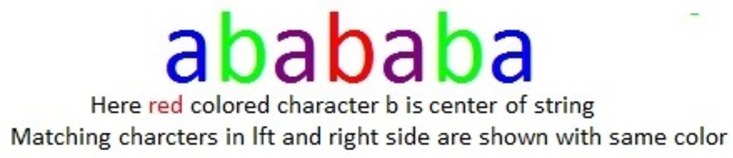
\includegraphics[width=0.5\textwidth]{Images/figGFGPalinManacher1}
%\caption[]{}
%\label{figCXNX}
\end{figure}

Here, center position is not only the actual string character position but it
could be the position between two characters also.  Consider string
\ctt{abaaba} of even length. This string is palindrome around the position
between $3$rd and $4$th characters \ctt{a} and \ctt{a} respectively.

\begin{figure}
\centering
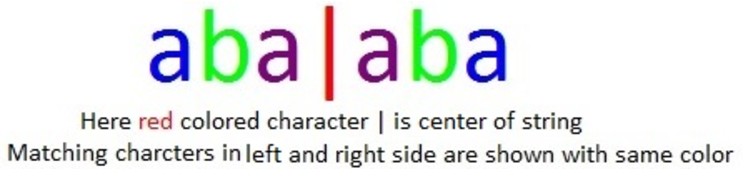
\includegraphics[width=0.5\textwidth]{Images/figGFGPalinManacher2}
%\caption[]{}
%\label{figCXNX}
\end{figure}

To find Longest Palindromic Substring of a string of length $N$, one way is
take each possible $2N+1$ centers (the $N$ character positions, $N-1$
between two character positions and $2$ positions at left and right ends),
do the character match in both left and right directions at each $2N+1$
centers and keep track of LPS. This approach takes $\comBigOh{N^2}$ time and
that's what we are doing in Set 2.

Let's consider two strings \ctt{abababa} and \ctt{abaaba} as shown below:

\begin{figure}
\centering
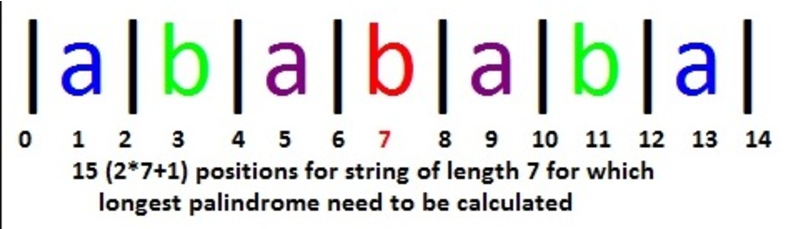
\includegraphics[width=0.5\textwidth]{Images/figGFGPalinManacher3}
%\caption[]{}
%\label{figCXNX}
\end{figure}

\begin{figure}
\centering
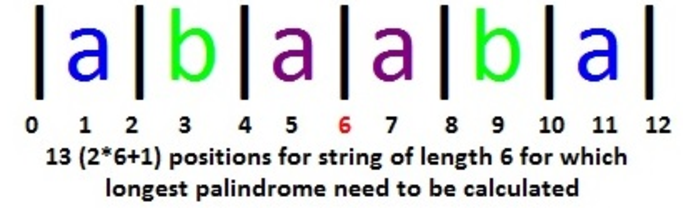
\includegraphics[width=0.5\textwidth]{Images/figGFGPalinManacher4}
%\caption[]{}
%\label{figCXNX}
\end{figure}

\rrblue{(Notice now if there is an odd number of chars, we add $N-1$ (even)
  $+2$ (even) for the end separators. This makes the total number of chars
  odd. If the number of chars is even, then we add an odd number of
  separators, again making the total number of chars even.)}

In these two strings, left and right side of the center positions (position
$7$ in $1$st string and position $6$ in $2$nd string) are symmetric. Why?
Because the whole string is palindrome around the center position.

If we need to calculate Longest Palindromic Substring at each $2N+1$
positions from left to right, then palindrome's symmetric property could
help to avoid some of the unnecessary computations (i.e. character
comparison). If there is a palindrome of some length $L$ centered at any
position $P$, then we may not need to compare all characters in left and
right side at position $P+1$. We already calculated LPS at positions before
$P$ and they can help to avoid \textbf{some} of the comparisons after
position $P$.

This use of information from previous positions at a later point of time
makes the Manacher's algorithm linear. In Set 2, there is no reuse of
previous information and so that is quadratic.

Manacher's algorithm is probably considered complex to understand, so here
we will discuss it in as detailed way as we can. Some of it's portions may
require multiple reading to understand it properly.

Let's look at string \ctt{abababa}. In 3rd figure above, 15 center positions
are shown. We need to calculate length of longest palindromic string at each
of these positions.
\begin{itemize}%[noitemsep,topsep=0pt]
\item At position $0$, there is no LPS at all (no character on left side to
  compare), so length of LPS will be $0$.
\item At position $1$, LPS is \ctt{a}, so length of LPS will be $1$.
\item At position $2$, there is no LPS at all (left and right characters
  \ctt{a} and \ctt{b} don't match), so length of LPS will be $0$.
\item At position $3$, LPS is \ctt{aba}, so length of LPS will be $3$.
\item At position $4$, there is no LPS at all (left and right characters
  \ctt{b} and \ctt{a} don't match), so length of LPS will be $0$.
\item At position $5$, LPS is \ctt{ababa}, so length of LPS will be $5$.
\end{itemize}
... and so on

We store all these palindromic lengths in an array, say $L$. Then string $S$
and LPS Length $L$ look like below:

\begin{figure}
\centering
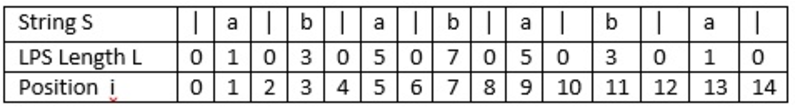
\includegraphics[width=0.7\textwidth]{Images/figGFGPalinManacher5}
%\caption[]{}
%\label{figCXNX}
\end{figure}

Similarly, LPS Length L of string \ctt{abaaba} will look like:

\begin{figure}
\centering
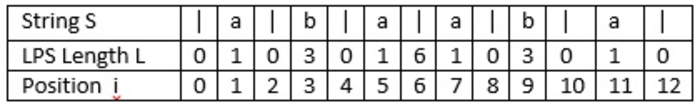
\includegraphics[width=0.7\textwidth]{Images/figGFGPalinManacher6}
%\caption[]{}
%\label{figCXNX}
\end{figure}

In LPS Array \ctt{L}:
\begin{itemize}%[noitemsep,topsep=0pt]
\item LPS length value at odd positions (the actual character positions)
  will be \textbf{odd} and \textbf{greater than or equal to 1} (1 will come
  from the center character itself if nothing else matches in left and right
  side of it) \rrblue{(It is odd because 1 will come from the center, and
    then we have characters on either side of the centre, total 1+even
    number of chars = odd number of chars)}
\item LPS length value at even positions (the positions between two
  characters, extreme left and right positions) will be even and greater
  than or equal to 0 (0 will come when there is no match in left and right
  side)
\end{itemize}
\begin{mdframed}[style=mdfNOTE]
\textbf{Position and index for the string are two different things here. For
  a given string $S$ of length $N$, indexes will be from $0$ to $N-1$ (total
  $N$ indexes) and positions will be from $0$ to $2N$ (total $2N+1$
  positions).}
\end{mdframed}

LPS length value can be interpreted in two ways, one in terms of index and
second in terms of position. LPS value $d$ at position $i$ ($L[i]=d$) tells
that:
\begin{itemize}%[noitemsep,topsep=0pt]
\item Substring from \textbf{position} $i-d$ to $i+d$ is a palindrome of
  length $d$ (in terms of position)
\item Substring from index $(i-d)/2$ to $[(i+d)/2-1]$ is a palindrome of
  length $d$ (in terms of index)
\end{itemize}
e.g. in string \ctt{abaaba}, \ctt{L[3]=3} means substring from position $0$
$(3-3)$ to $6$ $(3+3)$ is a palindrome which is \ctt{aba} of length $3$
\rrblue{(see red position numbers below)}, it also means that substring from
index $0$ $[(3-3)/2]$ to $2$ $[(3+3)/2-1]$ is a palindrome which is
\ctt{aba} of length $3$.

\begin{figure}
\centering
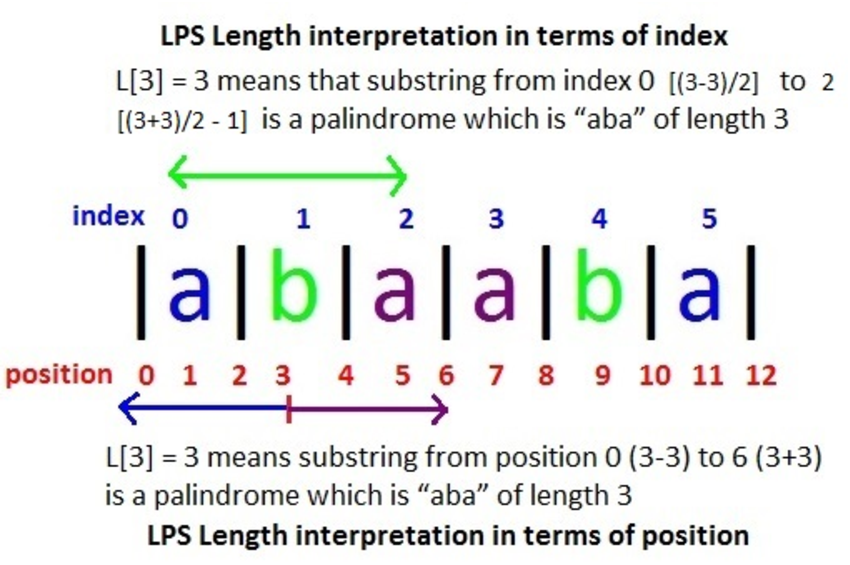
\includegraphics[width=0.7\textwidth]{Images/figGFGPalinManacher7}
%\caption[]{}
%\label{figCXNX}
\end{figure}

Now the main task is to compute LPS array efficiently. Once this array is
computed, LPS of string $S$ will be centered at position with maximum LPS
length value. We will see it in Part 2.

This article is contributed by Anurag Singh. Please write comments if you
find anything incorrect, or you want to share more information about the
topic discussed above

\RayNotesBegin

Okay, I give up for now. I just realised that this is in four parts.

\begin{itemize}%[noitemsep,topsep=0pt]
\item \url{todo}
\item \url{todo}
\item \url{todo}
\end{itemize}

\RayNotesEnd

%\textbf{\rrgreen{Recommended: Please try your approach first, before moving
%    on to the solution.}}
%
%\RayNotesBegin
%
%
%
%\RayNotesEnd
%
%\textbf{\rrgreen{Back to geeksforgeeks solution.}}



%%%%%%%%%%%%%%%%%%%%%%%%%%%%%%%%%%%%%%%%%%%%%%%%%%%%%%%%%%%%%%%%%%%%%%%%%%%%
%%%%%%%%%%%%%%%%%%%%%%%%%%%%%%%%%%%%%%%%%%%%%%%%%%%%%%%%%%%%%%%%%%%%%%%%%%%%
%%%%%%%%%%%%%%%%%%%%%%%%%%%%%%%%%%%%%%%%%%%%%%%%%%%%%%%%%%%%%%%%%%%%%%%%%%%%

\section{Manacher's Algorithm -- Linear Time Longest Palindromic Substring
  -- Part 2
  \label{secLPSStrGFGManacherPt2}}

\url{https://www.geeksforgeeks.org/manachers-algorithm-linear-time-longest-palindromic-substring-part-2}

\textbf{Difficulty: 4.4}

%In Manacher’s Algorithm – Part 1, we gone through some of the basics and LPS length array.
%Here we will see how to calculate LPS length array efficiently.
%
%To calculate LPS array efficiently, we need to understand how LPS length for any position may relate to LPS length value of any previous already calculated position.
%For string “abaaba”, we see following:
%
%\begin{figure}
%\centering
%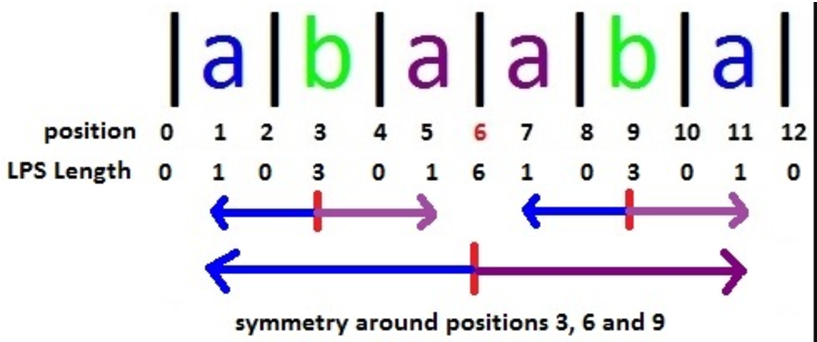
\includegraphics[width=0.7\textwidth]{Images/figGFGPalinManacher8}
%%\caption[]{}
%%\label{figCXNX}
%\end{figure}
%
%If we look around position 3:
%
%LPS length value at position 2 and position 4 are same
%LPS length value at position 1 and position 5 are same
%We calculate LPS length values from left to right starting from position 0, so we can see if we already know LPS length values at positions 1, 2 and 3 already then we may not need to calculate LPS length at positions 4 and 5 because they are equal to LPS length values at corresponding positions on left side of position 3.
%
%If we look around position 6:
%
%LPS length value at position 5 and position 7 are same
%LPS length value at position 4 and position 8 are same
%…………. and so on.
%If we already know LPS length values at positions 1, 2, 3, 4, 5 and 6 already then we may not need to calculate LPS length at positions 7, 8, 9, 10 and 11 because they are equal to LPS length values at corresponding positions on left side of position 6.
%
%For string “abababa”, we see following:
%
%\begin{figure}
%\centering
%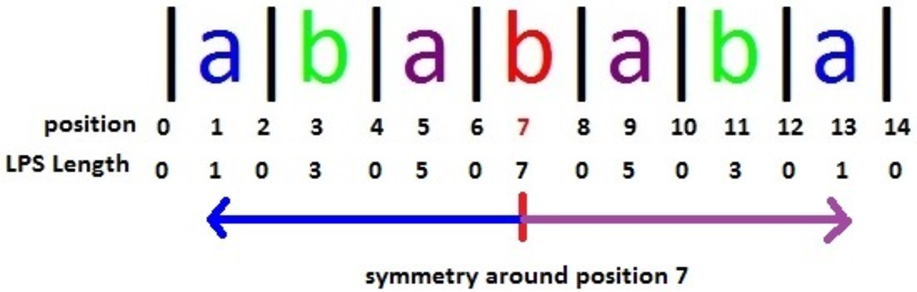
\includegraphics[width=0.7\textwidth]{Images/figGFGPalinManacher9}
%%\caption[]{}
%%\label{figCXNX}
%\end{figure}
%
%If we already know LPS length values at positions 1, 2, 3, 4, 5, 6 and 7 already then we may not need to calculate LPS length at positions 8, 9, 10, 11, 12 and 13 because they are equal to LPS length values at corresponding positions on left side of position 7.
%
%Can you see why LPS length values are symmetric around positions 3, 6, 9 in string “abaaba”? That’s because there is a palindromic substring around these positions. Same is the case in string “abababa” around position 7.
%Is it always true that LPS length values around at palindromic center position are always symmetric (same)?
%Answer is NO.
%Look at positions 3 and 11 in string “abababa”. Both positions have LPS length 3. Immediate left and right positions are symmetric (with value 0), but not the next one. Positions 1 and 5 (around position 3) are not symmetric. Similarly, positions 9 and 13 (around position 11) are not symmetric.
%
%At this point, we can see that if there is a palindrome in a string centered at some position, then LPS length values around the center position may or may not be symmetric depending on some situation. If we can identify the situation when left and right positions WILL BE SYMMETRIC around the center position, we NEED NOT calculate LPS length of the right position because it will be exactly same as LPS value of corresponding position on the left side which is already known. And this fact where we are avoiding LPS length computation at few positions makes Manacher’s Algorithm linear.
%
%In situations when left and right positions WILL NOT BE SYMMETRIC around the center position, we compare characters in left and right side to find palindrome, but here also algorithm tries to avoid certain no of comparisons. We will see all these scenarios soon.
%
%Let’s introduce few terms to proceed further:
%
%\begin{figure}
%\centering
%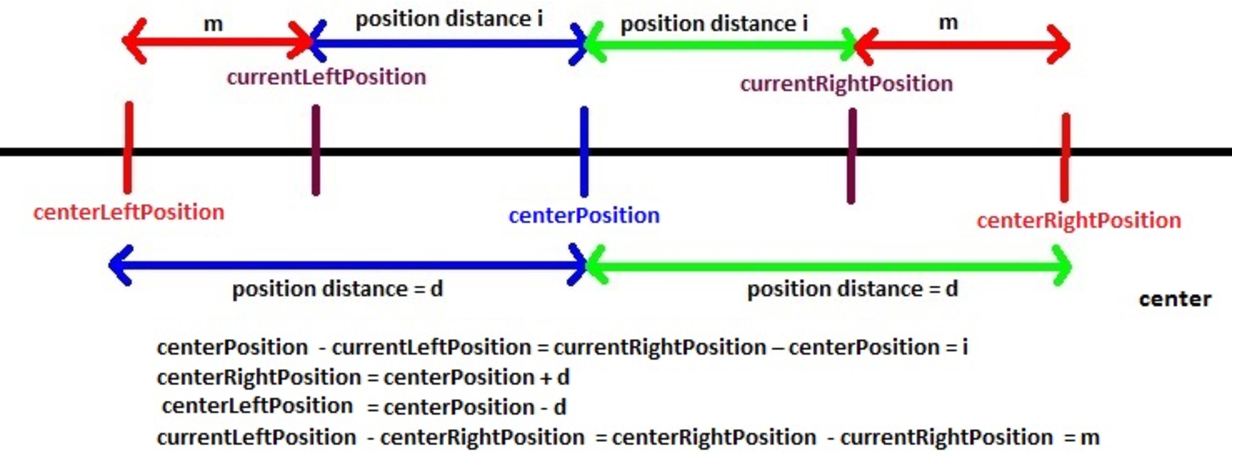
\includegraphics[width=0.7\textwidth]{Images/figGFGPalinManacher10}
%%\caption[]{}
%%\label{figCXNX}
%\end{figure}
%
%centerPosition – This is the position for which LPS length is calculated and let’s say LPS length at centerPosition is d (i.e. L[centerPosition] = d)
%centerRightPosition – This is the position which is right to the centerPosition and d position away from centerPosition (i.e. centerRightPosition = centerPosition + d)
%centerLeftPosition – This is the position which is left to the centerPosition and d position away from centerPosition (i.e. centerLeftPosition = centerPosition – d)
%currentRightPosition – This is the position which is right of the centerPosition for which LPS length is not yet known and has to be calculated
%currentLeftPosition – This is the position on the left side of centerPosition which corresponds to the currentRightPosition
%centerPosition – currentLeftPosition = currentRightPosition – centerPosition
%currentLeftPosition = 2* centerPosition – currentRightPosition
%i-left palindrome – The palindrome i positions left of centerPosition, i.e. at currentLeftPosition
%i-right palindrome – The palindrome i positions right of centerPosition, i.e. at currentRightPosition
%center palindrome – The palindrome at centerPosition
%When we are at centerPosition for which LPS length is known, then we also know LPS length of all positions smaller than centerPosition. Let’s say LPS length at centerPosition is d, i.e.
%L[centerPosition] = d
%
%It means that substring between positions “centerPosition-d” to “centerPosition+d” is a palindrom.
%Now we proceed further to calculate LPS length of positions greater than centerPosition.
%Let’s say we are at currentRightPosition ( > centerPosition) where we need to find LPS length.
%For this we look at LPS length of currentLeftPosition which is already calculated.
%
%If LPS length of currentLeftPosition is less than “centerRightPosition – currentRightPosition”, then LPS length of currentRightPosition will be equal to LPS length of currentLeftPosition. So
%L[currentRightPosition] = L[currentLeftPosition] if L[currentLeftPosition] < centerRightPosition – currentRightPosition. This is Case 1.
%
%Let’s consider below scenario for string “abababa”:
%
%\begin{figure}
%\centering
%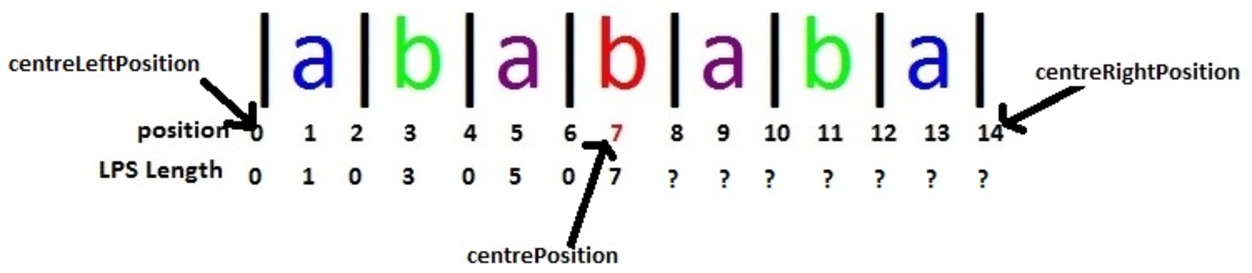
\includegraphics[width=0.7\textwidth]{Images/figGFGPalinManacher11}
%%\caption[]{}
%%\label{figCXNX}
%\end{figure}
%
%We have calculated LPS length up-to position 7 where L[7] = 7, if we consider position 7 as centerPosition, then centerLeftPosition will be 0 and centerRightPosition will be 14.
%Now we need to calculate LPS length of other positions on the right of centerPosition.
%
%For currentRightPosition = 8, currentLeftPosition is 6 and L[currentLeftPosition] = 0
%Also centerRightPosition – currentRightPosition = 14 – 8 = 6
%Case 1 applies here and so L[currentRightPosition] = L[8] = 0
%Case 1 applies to positions 10 and 12, so,
%L[10] = L[4] = 0
%L[12] = L[2] = 0
%
%If we look at position 9, then:
%currentRightPosition = 9
%currentLeftPosition = 2* centerPosition – currentRightPosition = 2*7 – 9 = 5
%centerRightPosition – currentRightPosition = 14 – 9 = 5
%
%Here L[currentLeftPosition] = centerRightPosition – currentRightPosition, so Case 1 doesn’t apply here. Also note that centerRightPosition is the extreme end position of the string. That means center palindrome is suffix of input string. In that case, L[currentRightPosition] = L[currentLeftPosition]. This is Case 2.
%
%Case 2 applies to positions 9, 11, 13 and 14, so:
%L[9] = L[5] = 5
%L[11] = L[3] = 3
%L[13] = L[1] = 1
%L[14] = L[0] = 0
%
%What is really happening in Case 1 and Case 2? This is just utilizing the palindromic symmetric property and without any character match, it is finding LPS length of new positions.
%
%When a bigger length palindrome contains a smaller length palindrome centered at left side of it’s own center, then based on symmetric property, there will be another same smaller palindrome centered on the right of bigger palindrome center. If left side smaller palindrome is not prefix of bigger palindrome, then Case 1 applies and if it is a prefix AND bigger palindrome is suffix of the input string itself, then Case 2 applies.
%
%The longest palindrome i places to the right of the current center (the i-right palindrome) is as long as the longest palindrome i places to the left of the current center (the i-left palindrome) if the i-left palindrome is completely contained in the longest palindrome around the current center (the center palindrome) and the i-left palindrome is not a prefix of the center palindrome (Case 1) or (i.e. when i-left palindrome is a prefix of center palindrome) if the center palindrome is a suffix of the entire string (Case 2).
%
%In Case 1 and Case 2, i-right palindrome can’t expand more than corresponding i-left palindrome (can you visualize why it can’t expand more?), and so LPS length of i-right palindrome is exactly same as LPS length of i-left palindrome.
%
%Here both i-left and i-right palindromes are completely contained in center palindrome (i.e. L[currentLeftPosition] <= centerRightPosition – currentRightPosition)
%Now if i-left palindrome is not a prefix of center palindrome (L[currentLeftPosition] < centerRightPosition – currentRightPosition), that means that i-left palindrome was not able to expand up-to position centerLeftPosition.
%
%If we look at following with centerPosition = 11, then
%
%\begin{figure}
%\centering
%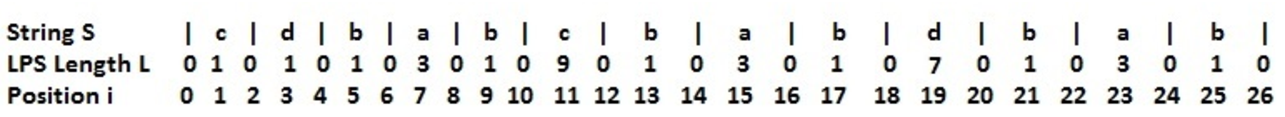
\includegraphics[width=0.7\textwidth]{Images/figGFGPalinManacher12}
%%\caption[]{}
%%\label{figCXNX}
%\end{figure}
%
%centerLeftPosition would be 11 – 9 = 2, and centerRightPosition would be 11 + 9 = 20
%If we take currentRightPosition = 15, it’s currentLeftPosition is 7. Case 1 applies here and so L[15] = 3. i-left palindrome at position 7 is “bab” which is completely contained in center palindrome at position 11 (which is “dbabcbabd”). We can see that i-right palindrome (at position 15) can’t expand more than i-left palindrome (at position 7).
%
%If there was a possibility of expansion, i-left palindrome could have expanded itself more already. But there is no such possibility as i-left palindrome is prefix of center palindrome. So due to symmetry property, i-right palindrome will be exactly same as i-left palindrome and it can’t expand more. This makes L[currentRightPosition] = L[currentLeftPosition] in Case 1.
%
%Now if we consider centerPosition = 19, then centerLeftPosition = 12 and centerRightPosition = 26
%If we take currentRightPosition = 23, it’s currentLeftPosition is 15. Case 2 applies here and so L[23] = 3. i-left palindrome at position 15 is “bab” which is completely contained in center palindrome at position 19 (which is “babdbab”). In Case 2, where i-left palindrome is prefix of center palindrome, i-right palindrome can’t expand more than length of i-left palindrome because center palindrome is suffix of input string so there are no more character left to compare and expand. This makes L[currentRightPosition] = L[currentLeftPosition] in Case 2.
%
%Case 1: L[currentRightPosition] = L[currentLeftPosition] applies when:
%
%i-left palindrome is completely contained in center palindrome
%i-left palindrome is NOT a prefix of center palindrome
%Both above conditions are satisfied when
%L[currentLeftPosition] < centerRightPosition – currentRightPosition
%
%Case 2: L[currentRightPosition] = L[currentLeftPosition] applies when:
%
%i-left palindrome is prefix of center palindrome (means completely contained also)
%center palindrome is suffix of input string
%Above conditions are satisfied when
%L[currentLeftPosition] = centerRightPosition – currentRightPosition (For 1st condition) AND
%centerRightPosition = 2*N where N is input string length N (For 2nd condition).
%
%Case 3: L[currentRightPosition] > = L[currentLeftPosition] applies when:
%
%i-left palindrome is prefix of center palindrome (and so i-left palindrome is completely contained in center palindrome)
%center palindrome is NOT suffix of input string
%Above conditions are satisfied when
%L[currentLeftPosition] = centerRightPosition – currentRightPosition (For 1st condition) AND
%centerRightPosition < 2*N where N is input string length N (For 2nd condition).
%In this case, there is a possibility of i-right palindrome expansion and so length of i-right palindrome is at least as long as length of i-left palindrome.
%
%Case 4: L[currentRightPosition] > = centerRightPosition – currentRightPosition applies when:
%
%i-left palindrome is NOT completely contained in center palindrome
%Above condition is satisfied when
%L[currentLeftPosition] > centerRightPosition – currentRightPosition
%In this case, length of i-right palindrome is at least as long (centerRightPosition – currentRightPosition) and there is a possibility of i-right palindrome expansion.
%
%In following figure,
%
%\begin{figure}
%\centering
%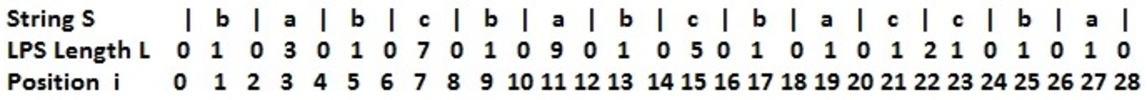
\includegraphics[width=0.7\textwidth]{Images/figGFGPalinManacher13}
%%\caption[]{}
%%\label{figCXNX}
%\end{figure}
%
%If we take center position 7, then Case 3 applies at currentRightPosition 11 because i-left palindrome at currentLeftPosition 3 is a prefix of center palindrome and i-right palindrome is not suffix of input string, so here L[11] = 9, which is greater than i-left palindrome length L[3] = 3. In the case, it is guaranteed that L[11] will be at least 3, and so in implementation, we 1st set L[11] = 3 and then we try to expand it by comparing characters in left and right side starting from distance 4 (As up-to distance 3, it is already known that characters will match).
%
%If we take center position 11, then Case 4 applies at currentRightPosition 15 because L[currentLeftPosition] = L[7] = 7 > centerRightPosition – currentRightPosition = 20 – 15 = 5. In the case, it is guaranteed that L[15] will be at least 5, and so in implementation, we 1st set L[15] = 5 and then we try to expand it by comparing characters in left and right side starting from distance 5 (As up-to distance 5, it is already known that characters will match).
%
%Now one point left to discuss is, when we work at one center position and compute LPS lengths for different rightPositions, how to know that what would be next center position. We change centerPosition to currentRightPosition if palindrome centered at currentRightPosition expands beyond centerRightPosition.
%
%Here we have seen four different cases on how LPS length of a position will depend on a previous position’s LPS length.
%In Part 3, we have discussed code implementation of it and also we have looked at these four cases in a different way and implement that too.
%
%This article is contributed by Anurag Singh. Please write comments if you find anything incorrect, or you want to share more information about the topic discussed above
%
%
%I give up, there's actually a part 3 and part four:
%
%https://www.geeksforgeeks.org/manachers-algorithm-linear-time-longest-palindromic-substring-part-3-2/
%
%https://www.geeksforgeeks.org/manachers-algorithm-linear-time-longest-palindromic-substring-part-4/
%


















\textbf{\rrgreen{Recommended: Please try your approach first, before moving
    on to the solution.}}

\RayNotesBegin



\RayNotesEnd

\textbf{\rrgreen{Back to geeksforgeeks solution.}}










